\section{Experiments}\label{sec:experiments}
We put into action and assessed the outcomes of pose estimation for both synthetic and real data employing both the fundamental matrix and the trifocal tensor. \footnote{The MATLAB code to reproduce these experiments is available at the GitHub repository: \href{https://github.com/versi379/Two-View-Three-View-Pose-Estimation.git}{https://github.com/versi379/Two-View-Three-View-Pose-Estimation.git}.} In the initial scenario, we employ linear computation for the tensor (\textbf{Linear TFT}) and apply Gauss-Helmert optimization using minimal parameterizations proposed by Ressl (\textbf{Ressl TFT}), Nordberg (\textbf{Nordberg TFT}), Faugeras and Papadopoulo (\textbf{Faugeras-Papadopoulo TFT}), and Ponce and Hebert (\textbf{Ponce-Hebert TFT}). As for the fundamental matrix, we compute it both linearly (\textbf{Linear FM}) and through Gauss-Helmert optimization (\textbf{Optimized FM}). Additionally, we present the result obtained through Bundle Adjustment (BA), which is initialized using any of the aforementioned methods. Remarkably, our experiments reveal that all initializations yield nearly identical final poses post-minimization in the majority of cases, an observation we delve into later in our discussions.

\subsection{Synthetic Data}
We conducted trials on synthetic data to assess pose estimation using both the fundamental matrix and the trifocal tensor across various configurations. The standard experimental setup consists of a collection of spatial points situated within a 400mm-sided cube centered at the world's origin (Figure X). Points are projected onto three views, and Gaussian noise with a standard deviation of 1 pixel is applied to the image points, unless specified otherwise. A set of 10 points is utilized for computations across various models. The image dimensions are \( 1800 \times 1200 \) pixels, representing a sensor size of \( 36mm \times 24mm \), with a fixed focal length of 50mm. All cameras are aligned to focus on the origin. Results are averaged over 30 simulations of data.\\

Overall, the experiments consistently demonstrate that pose estimation derived from the trifocal tensor outperforms that based on the fundamental matrix. Regardless of the method used to optimize the trifocal tensor with minimal parameterization, each effectively enhances the initial linear solution, converging to the same minimum. Similarly, optimizing the fundamental matrix reduces the error of the linear solution. Despite these enhancements being evident, they do not affect the minimum attained through Bundle Adjustment, which is achieved even when initialized by the most basic method (\ie, linear fundamental matrix estimation).\\

% Varying noise discussion
Metrics before and after Bundle Adjustment, against Gaussian noise level added to the data points, are shown respectively in Figure (\ref{fig:initNoisePlot}) and Figure (\ref{fig:BANoisePlot}).\\

% Varying focal length discussion
Metrics before and after Bundle Adjustment, against the varying focal length, are shown respectively in Figure (\ref{fig:initFocalPlot}) and Figure (\ref{fig:BAFocalPlot}).\\

% Varying number of points discussion
Metrics before and after Bundle Adjustment, against the number of points considered in the synthetic scene, are shown respectively in Figure (\ref{fig:initPointsPlot}) and Figure (\ref{fig:BAPointsPlot}).\\

% Varying angle discussion
Metrics before and after Bundle Adjustment, against the varying angle among the three camera centers, are shown respectively in Figure (\ref{fig:initAnglePlot}) and Figure (\ref{fig:BAAnglePlot}).

\begin{figure}[p]
	\centering
	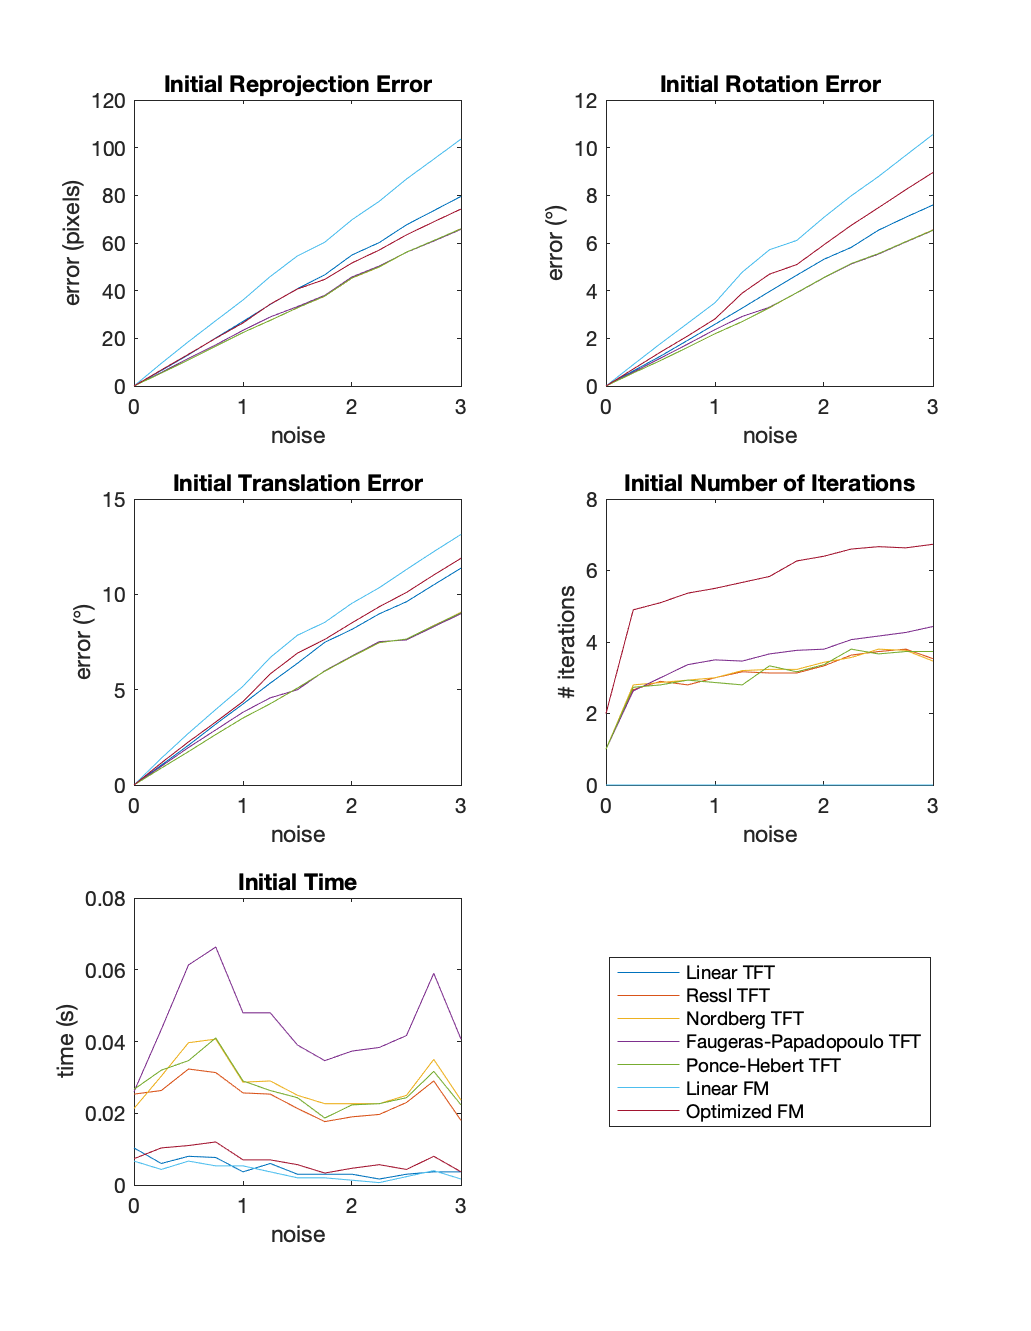
\includegraphics[width=1\textwidth]{Experiments/Synthetic/noise/INITnoisePlots.png}
	\caption{Initial reprojection error (top-left), rotation error (top-right), translation error (mid-left), number of iterations (mid-right), computational time (bottom-left); when varying the Gaussian noise added to the image points.}
	\label{fig:initNoisePlot}
\end{figure}

\begin{figure}[p]
	\centering
	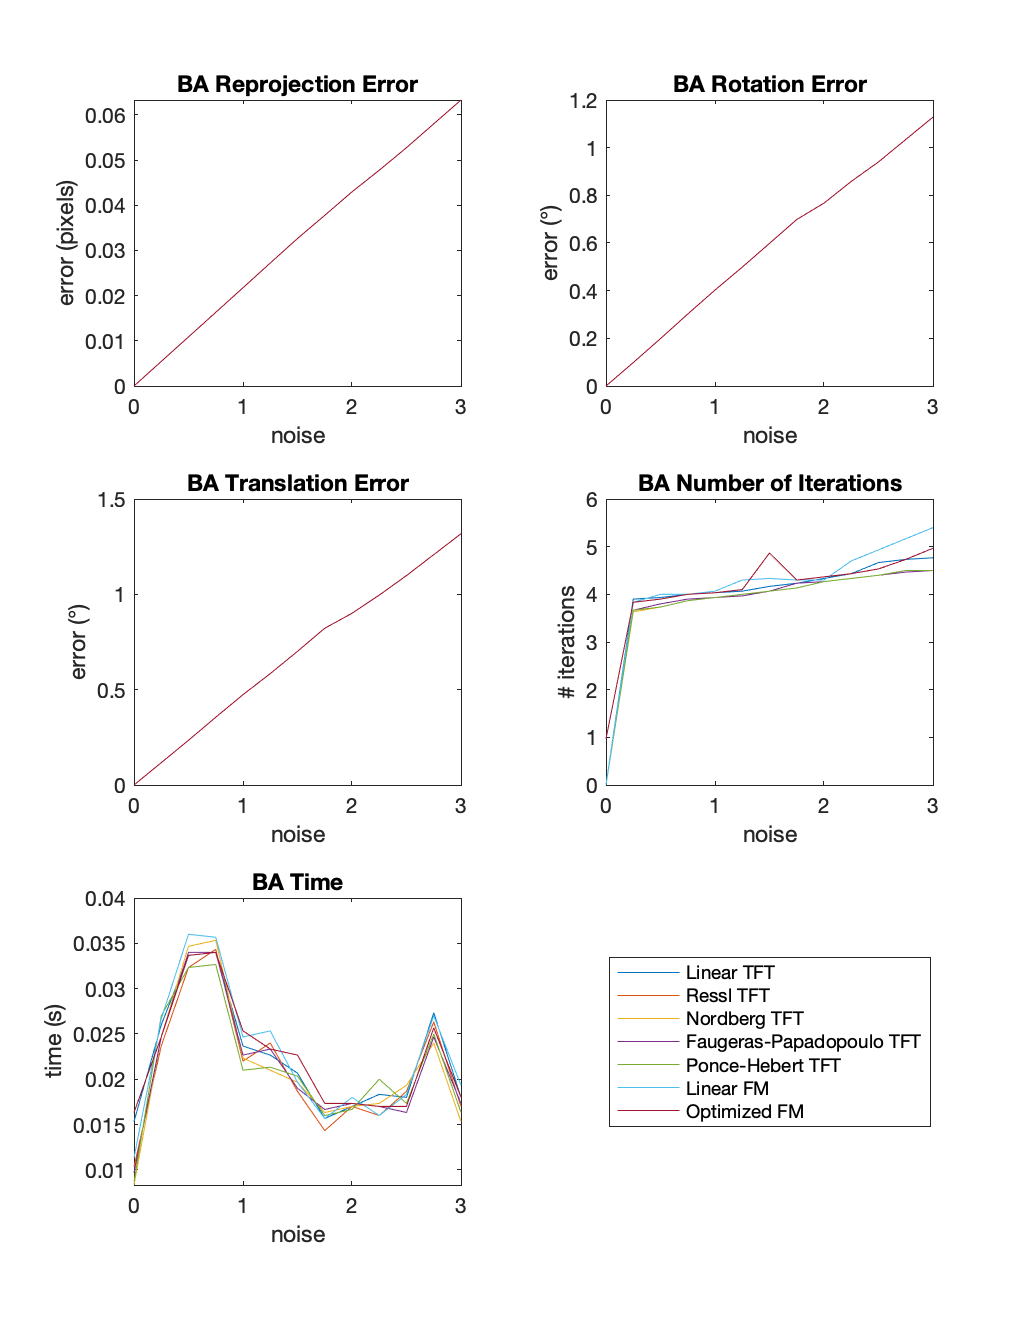
\includegraphics[width=1\textwidth]{Experiments/Synthetic/noise/BAnoisePlots.png}
	\caption{Reprojection error (top-left), rotation error (top-right), translation error (mid-left), number of iterations (mid-right), computational time (bottom-left) after Bundle Adjustment; when varying the focal length.}
	\label{fig:BANoisePlot}
\end{figure}

\begin{figure}[p]
	\centering
	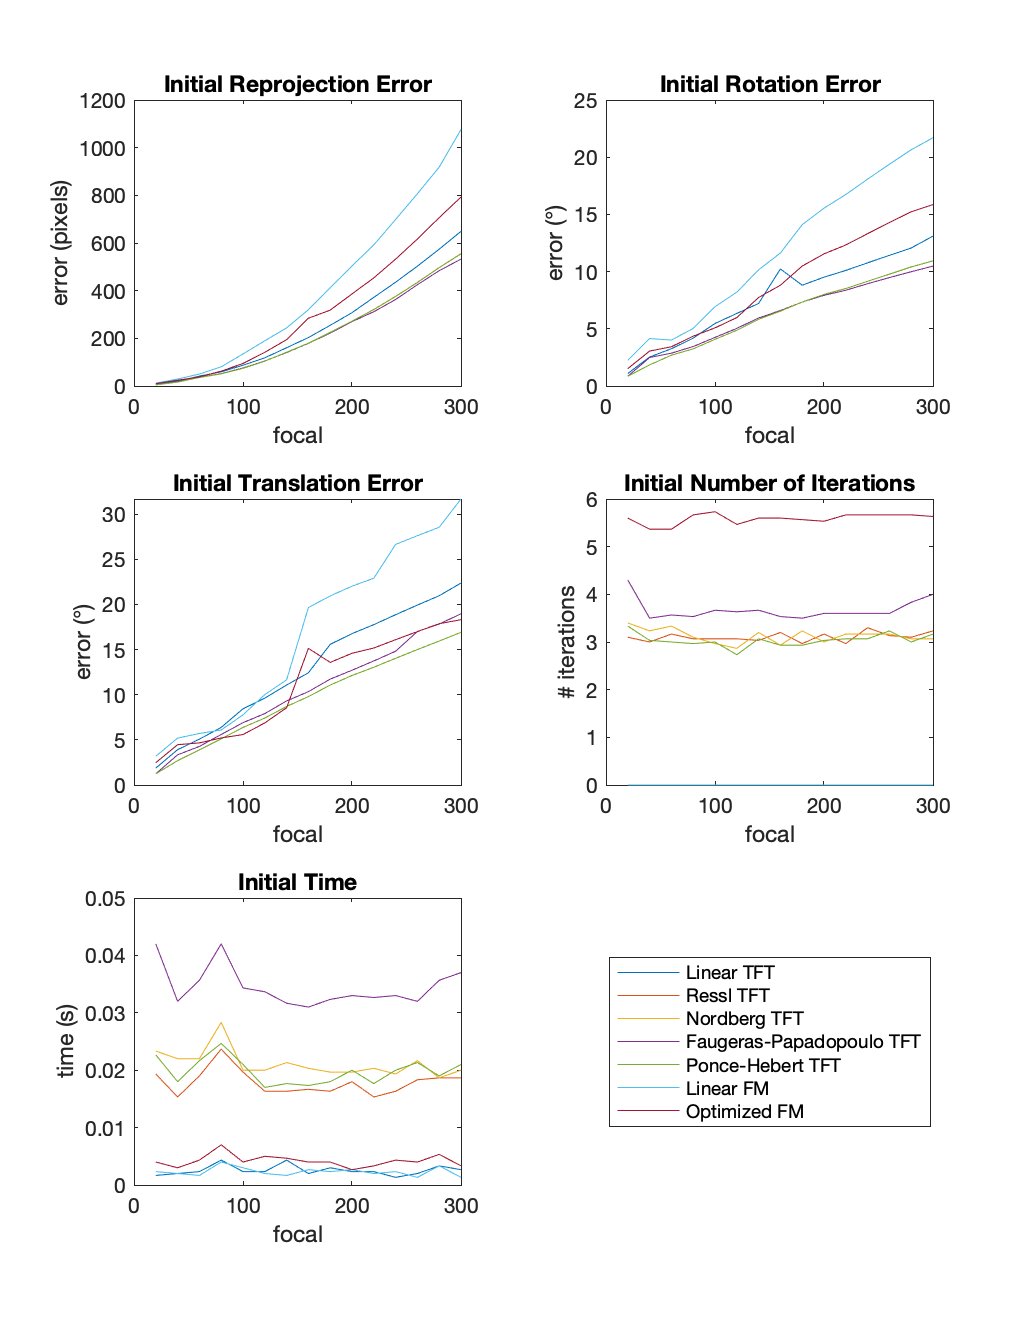
\includegraphics[width=1\textwidth]{Experiments/Synthetic/focal/INITfocalPlots.png}
	\caption{Initial reprojection error (top-left), rotation error (top-right), translation error (mid-left), number of iterations (mid-right), computational time (bottom-left); when varying the Gaussian noise added to the image points.}
	\label{fig:initFocalPlot}
\end{figure}

\begin{figure}[p]
	\centering
	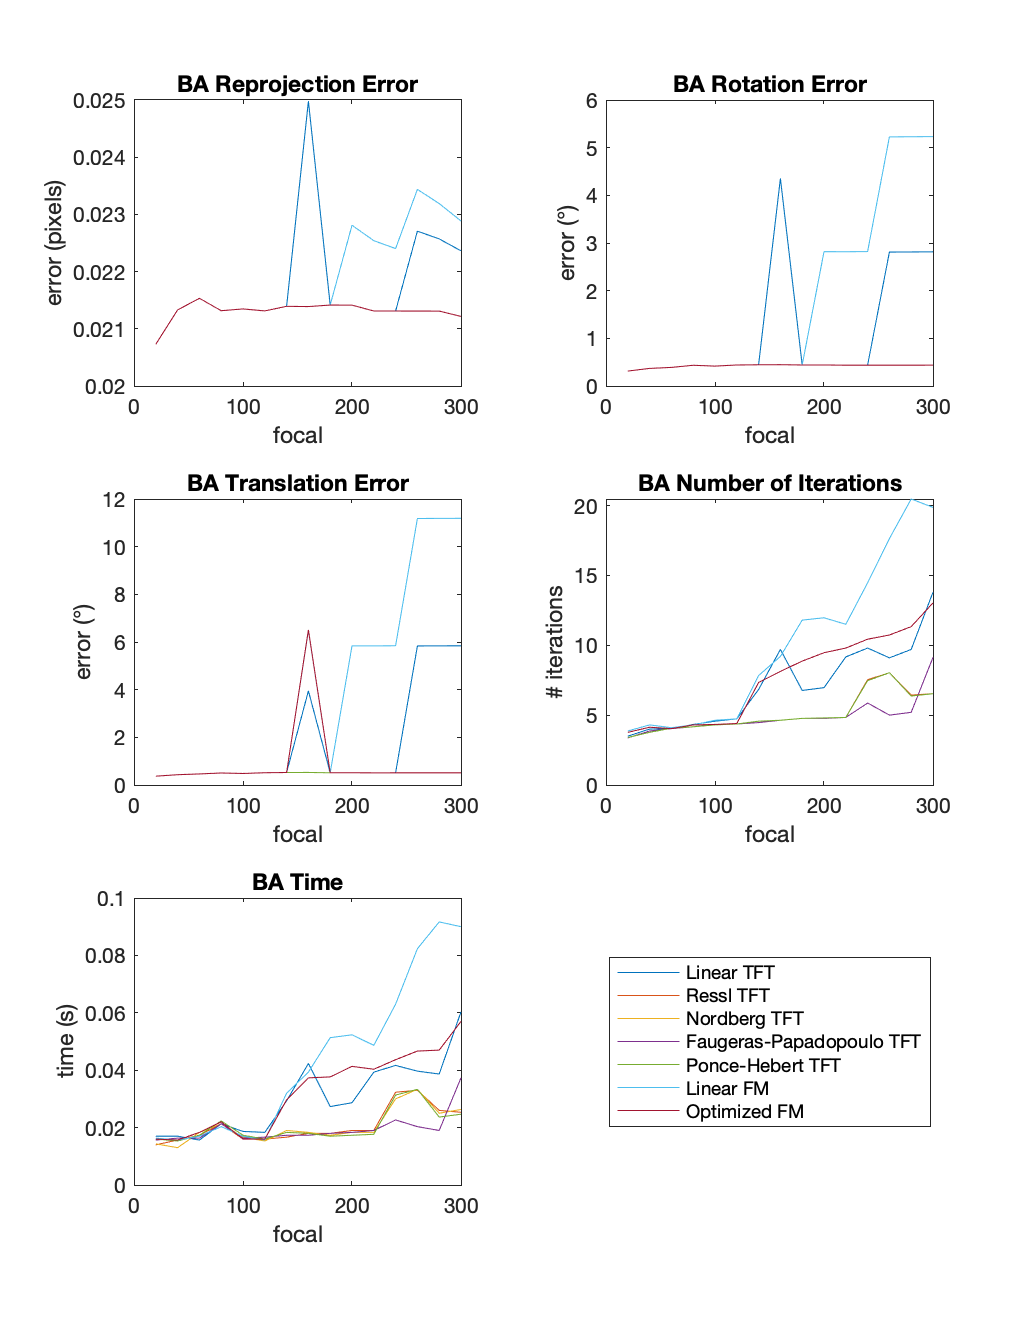
\includegraphics[width=1\textwidth]{Experiments/Synthetic/focal/BAfocalPlots.png}
	\caption{Reprojection error (top-left), rotation error (top-right), translation error (mid-left), number of iterations (mid-right), computational time (bottom-left) after Bundle Adjustment; when varying the focal length.}
	\label{fig:BAFocalPlot}
\end{figure}

\begin{figure}[p]
	\centering
	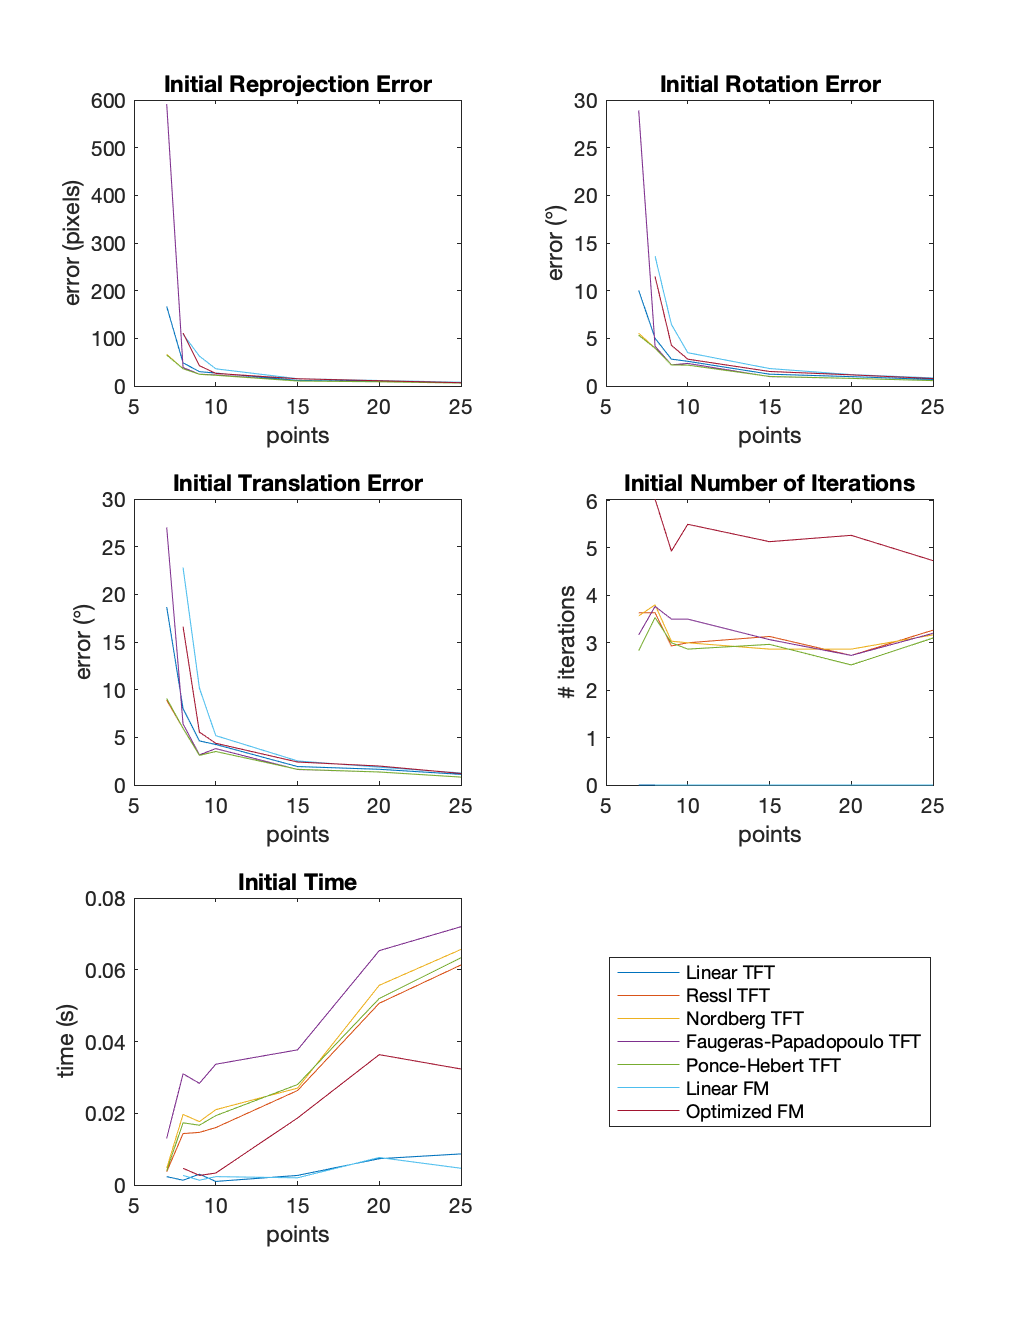
\includegraphics[width=1\textwidth]{Experiments/Synthetic/points/INITpointsPlots.png}
	\caption{Initial reprojection error (top-left), rotation error (top-right), translation error (mid-left), number of iterations (mid-right), computational time (bottom-left); when varying the number of image points.}
	\label{fig:initPointsPlot}
\end{figure}

\begin{figure}[p]
	\centering
	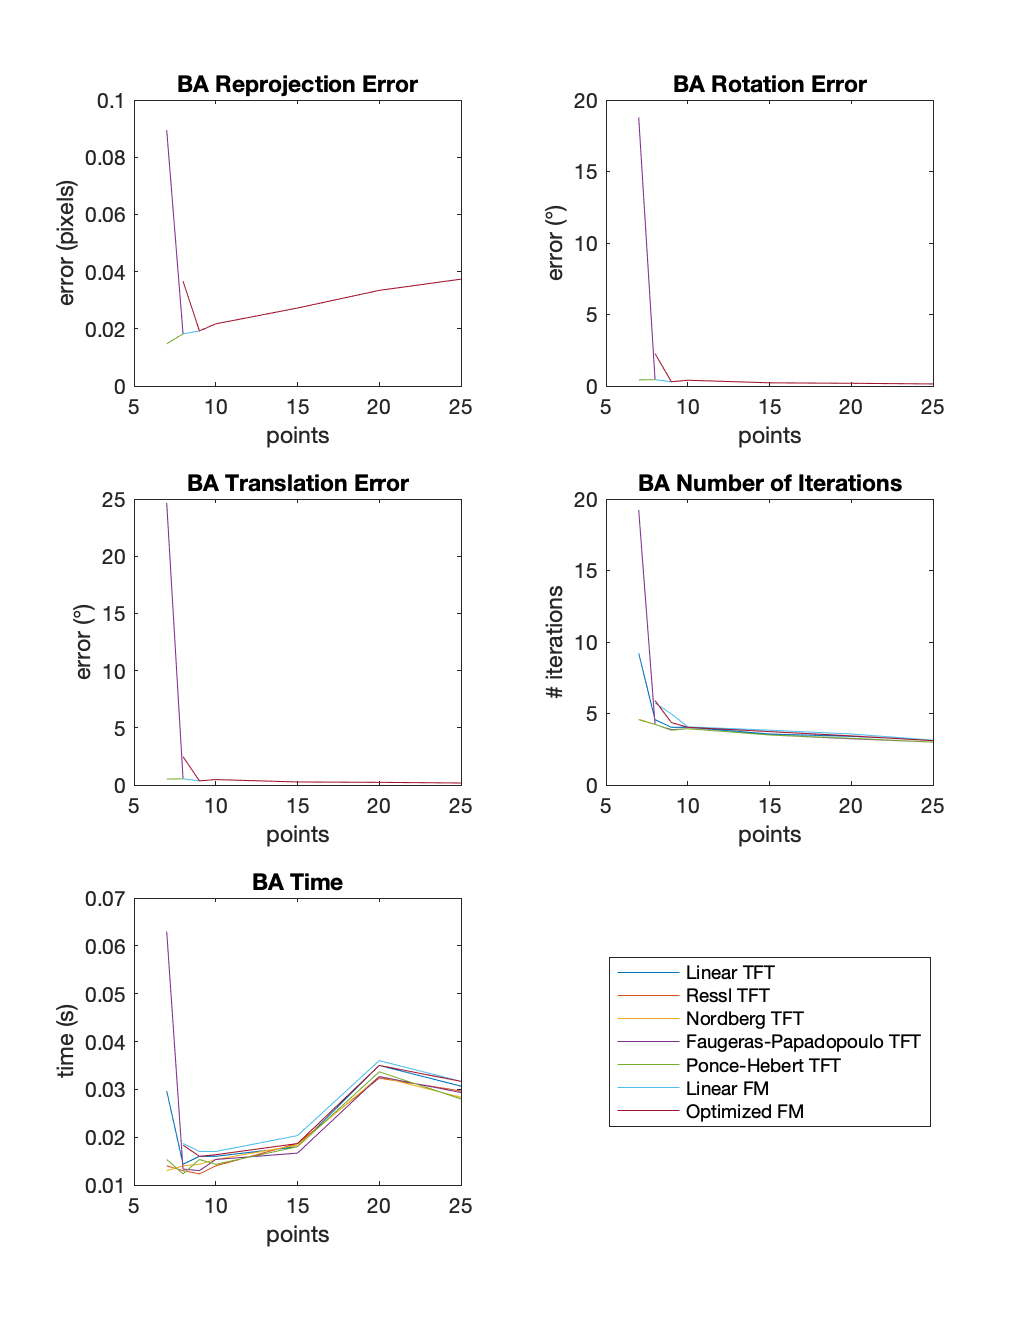
\includegraphics[width=1\textwidth]{Experiments/Synthetic/points/BApointsPlots.png}
	\caption{Reprojection error (top-left), rotation error (top-right), translation error (mid-left), number of iterations (mid-right), computational time (bottom-left) after Bundle Adjustment; when varying the number of image points.}
	\label{fig:BAPointsPlot}
\end{figure}

\begin{figure}[p]
	\centering
	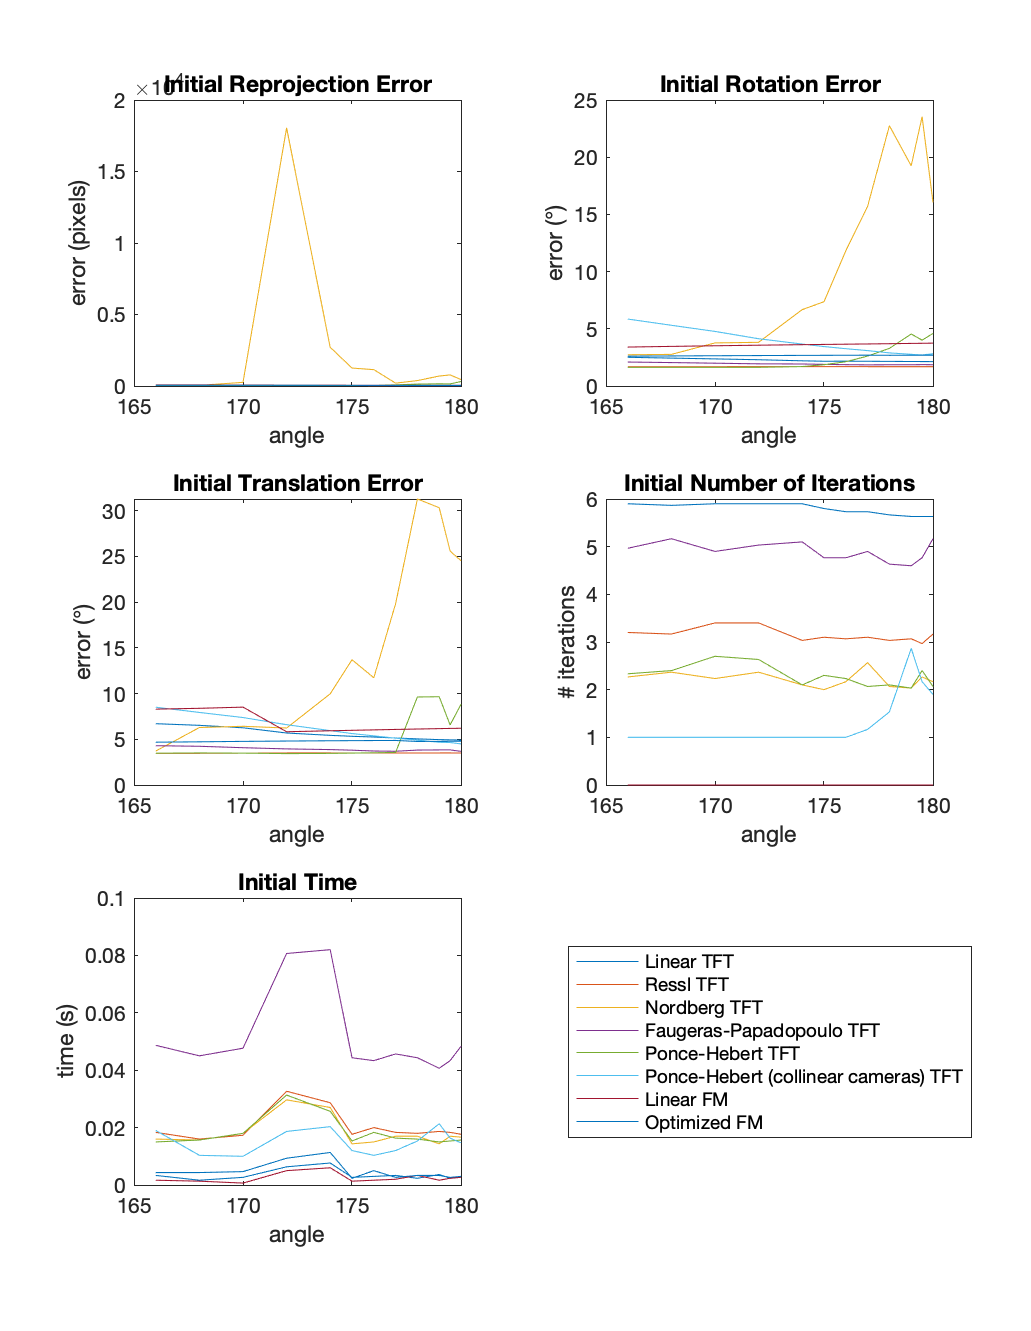
\includegraphics[width=1\textwidth]{Experiments/Synthetic/angle/INITanglePlots.png}
	\caption{Initial reprojection error (top-left), rotation error (top-right), translation error (mid-left), number of iterations (mid-right), computational time (bottom-left); when varying the angle among the three camera centers.}
	\label{fig:initAnglePlot}
\end{figure}

\begin{figure}[p]
	\centering
	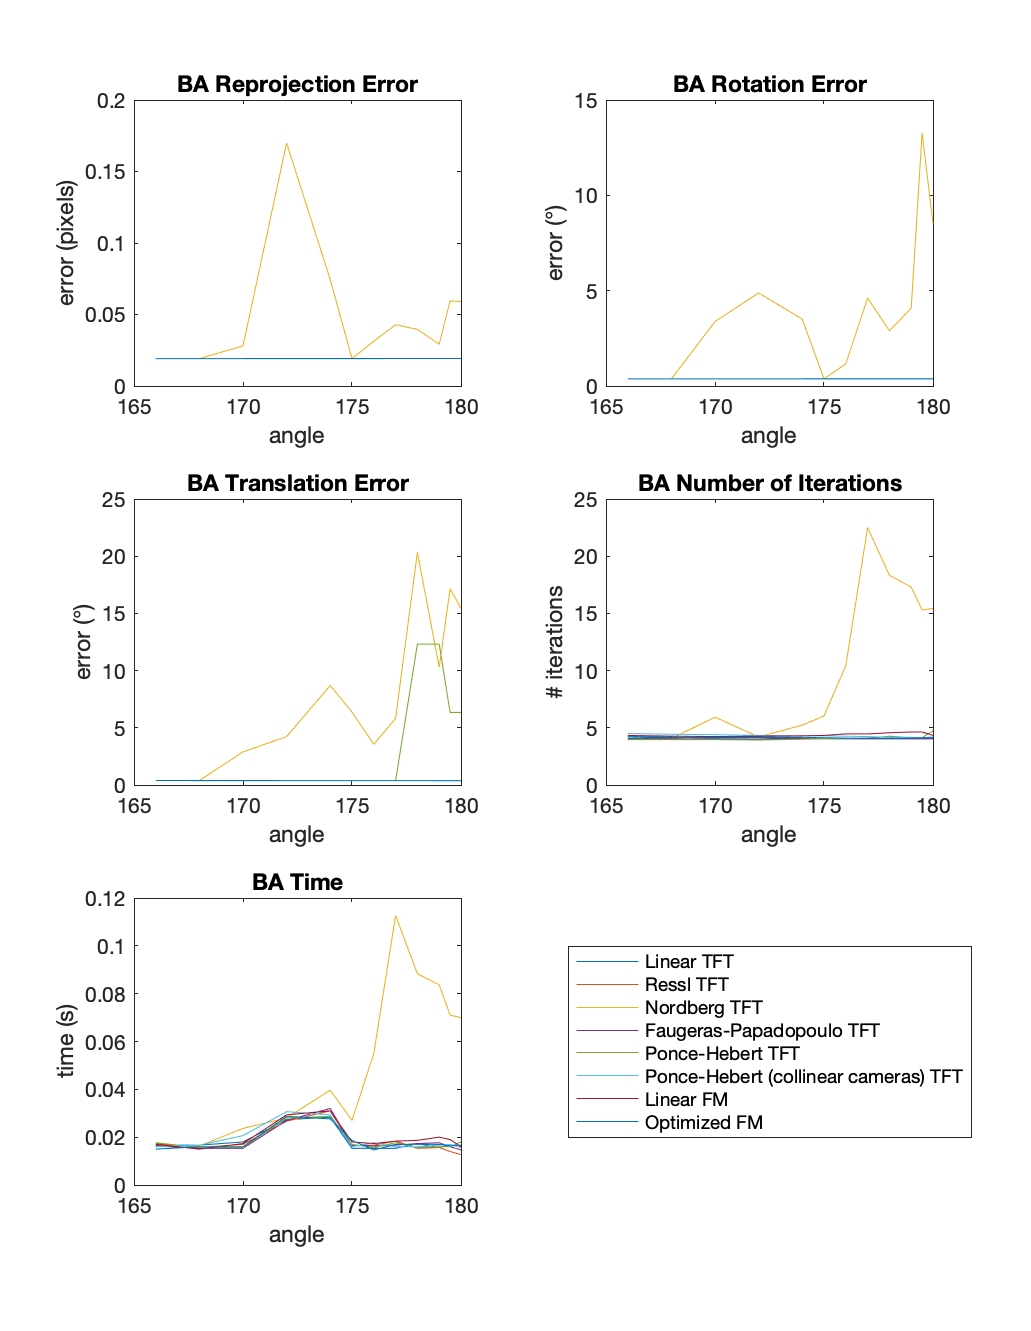
\includegraphics[width=1\textwidth]{Experiments/Synthetic/angle/BAanglePlots.png}
	\caption{Reprojection error (top-left), rotation error (top-right), translation error (mid-left), number of iterations (mid-right), computational time (bottom-left) after Bundle Adjustment; when varying the angle among the three camera centers.}
	\label{fig:BAAnglePlot}
\end{figure}

\pagebreak

\subsection{Real Data}
In assessing the efficacy of these methods within real-world contexts, we opted to utilize scenes from the EPFL Dense Multi-View Stereo Dataset, presented in \cite{13-epfl-dataset}, provided by the CVLab at EPFL. \footnote{The EPFL Dense Multi-View Stereo Dataset, featuring the scenes utilized in our study, is readily accessible at the following location: \href{https://documents.epfl.ch/groups/c/cv/cvlab-unit/www/data/multiview/denseMVS.html}{https://documents.epfl.ch/groups/c/cv/cvlab-unit/www/data/multiview/denseMVS.html}.}\\

Table (\ref{tab:fountainInit}) and (\ref{tab:fountainBA}) show metrics before and after Bundle Adjustment with respect to the \textit{fountain-P11} set of images from the dataset.

\begin{table}[htbp]
  \centering
  \caption{Initial metrics with respect to the \textit{fountain-P11} set of images.}
  \label{tab:fountainInit}
  \begin{tabular}{|*{6}{c}|}
    \hline
     & repr. error (px) & R error ($^{\circ}$) & t error ($^{\circ}$) & \# iter. & time (s)\\
    \hline
    \textbf{Linear TFT} & 2.3953 & 0.1249 & 0.4048 & 0 & 0.0621 \\
    \textbf{Ressl TFT} & 2.0474 & 0.1158 & 0.4003 & 2.8429 & 0.6400 \\
    \textbf{Nordberg TFT} & 2.1322 & 0.1334 & 0.4028 & 2.8000 & 0.6280 \\
    \textbf{Faugeras-Papadopoulo TFT} & 2.3688 & 0.1187 & 0.4055 & 2.7714 & 0.6073 \\
    \textbf{Ponce-Hebert TFT} & 2.0871 & 0.1167 & 0.4030 & 2.5857 & 0.5554 \\
    \textbf{Linear FM} & 1.9671 & 0.1149 & 0.3717 & 0 & 0.0273 \\
    \textbf{Optimized FM} & 1.9530 & 0.1127 & 0.3658 & 4.9286 & 0.3209 \\
    \hline
  \end{tabular}
\end{table}

\begin{table}[htbp]
  \centering
  \caption{Metrics after Bundle Adjustment with respect to the \textit{fountain-P11} set of images.}
  \label{tab:fountainBA}
  \begin{tabular}{|*{6}{c}|}
    \hline
     & repr. error (px) & R error ($^{\circ}$) & t error ($^{\circ}$) & \# iter. & time (s)\\
     \hline
    \textbf{Linear TFT} & 0.2814 & 0.0640 & 0.0743 & 3.8143 & 0.0743 \\
    \textbf{Ressl TFT} & 0.2814 & 0.0640 & 0.0743 & 3.8286 & 0.0720 \\
    \textbf{Nordberg TFT} & 0.2814 & 0.0640 & 0.0743 & 3.8571 & 0.0716 \\
    \textbf{Faugeras-Papadopoulo TFT} & 0.2814 & 0.0640 & 0.0743 & 3.8429 & 0.0723 \\
    \textbf{Ponce-Hebert TFT} & 0.2814 & 0.0640 & 0.0743 & 3.8429 & 0.0743 \\
    \textbf{Linear FM} & 0.2814 & 0.0640 & 0.0743 & 3.7714 & 0.0816 \\
    \textbf{Optimized FM} & 0.2814 & 0.0640 & 0.0743 & 3.8000 & 0.0784 \\
    \hline
  \end{tabular}
\end{table}

Table (\ref{tab:HerzJesuInit}) and (\ref{tab:HerzJesuBA}) show metrics before and after Bundle Adjustment with respect to the \textit{Herz-Jesu-P8} set of images from the dataset.

\begin{table}[htbp]
  \centering
  \caption{Initial metrics with respect to the \textit{Herz-Jesu-P8} set of images.}
  \label{tab:HerzJesuInit}
  \begin{tabular}{|*{6}{c}|}
    \hline
     & repr. error (px) & R error ($^{\circ}$) & t error ($^{\circ}$) & \# iter. & time (s)\\
    \hline
    \textbf{Linear TFT} & 4.8062 & 0.4589 & 0.8707 & 0 & 0.0506 \\
    \textbf{Ressl TFT} & 3.4792 & 0.3966 & 0.6677 & 2.7800 & 0.4904 \\
    \textbf{Nordberg TFT} & 4.0656 & 0.5252 & 0.6917 & 2.6600 & 0.4816 \\
    \textbf{Faugeras-Papadopoulo TFT} & 4.5006 & 0.4459 & 0.8324 & 3.4400 & 0.5452 \\
    \textbf{Ponce-Hebert TFT} & 4.5293 & 0.4261 & 0.6682 & 2.3000 & 0.4116 \\
    \textbf{Linear FM} & 3.7624 & 0.4142 & 0.7725 & 0 & 0.0224 \\
    \textbf{Optimized FM} & 3.6503 & 0.4196 & 0.7654 & 5.6600 & 0.2906 \\
    \hline
  \end{tabular}
\end{table}

\begin{table}[htbp]
  \centering
  \caption{Metrics after Bundle Adjustment with respect to the \textit{Herz-Jesu-P8} set of images.}
  \label{tab:HerzJesuBA}
  \begin{tabular}{|*{6}{c}|}
    \hline
     & repr. error (px) & R error ($^{\circ}$) & t error ($^{\circ}$) & \# iter. & time (s)\\
    \hline
    \textbf{Linear TFT} & 0.3719 & 0.0635 & 0.0682 & 4.0600 & 0.0792 \\
    \textbf{Ressl TFT} & 0.3719 & 0.0635 & 0.0682 & 4.0000 & 0.0674 \\
    \textbf{Nordberg TFT} & 0.3719 & 0.0635 & 0.0682 & 4.0400 & 0.0690 \\
    \textbf{Faugeras-Papadopoulo TFT} & 0.3719 & 0.0635 & 0.0682 & 4.0600 & 0.0680 \\
    \textbf{Ponce-Hebert TFT} & 0.3719 & 0.0635 & 0.0682 & 4.0000 & 0.0664 \\
    \textbf{Linear FM} & 0.3719 & 0.0635 & 0.0682 & 4.0000 & 0.0718 \\
    \textbf{Optimized FM} & 0.3719 & 0.0635 & 0.0682 & 4.0200 & 0.0724 \\
    \hline
  \end{tabular}
\end{table}

\pagebreak
